\chapter{Methodik}
\label{sec.Methodik}
Dieses Kapitel behandelt die Methodik zur Prädiktion von Umweltzuständen. Die Beschreibung der verwendeten Methoden erfolgt separat für binäre Zustandsmodelle (Abschnitt \ref{sec.Binäre Zustandsmodelle}), bei denen die Wahrscheinlichkeit $p(t)$ für einen Umweltzustand, wie beispielsweise die Belegtheit $s(t)$ einer Zelle innerhalb eines geografischen Gitters, bestimmt werden soll, sowie für quantitative Zustandsmodelle (Abschnitt \ref{sec.Quantitative Zustandsmodelle}), bei denen Aussagen über die Anzahl an Ereignissen innerhalb einer Zelle während eines bestimmten Zeitintervalls getroffen werden sollen.
\section{Binäre Zustandsmodelle}
\label{sec.Binäre Zustandsmodelle}
Binäre Zustandsmodelle dienen, wie schon in Abschnitt \ref{sec.Beschreibung quantitativer Zustandsmodelle} erläutert, der Beschreibung einer Zustandsfunktion $s(t)$ durch eine Wahrscheinlichkeitsfunktion $p(t)$. In den folgenden Abschnitten werden die Schritte zur Bestimmung dieser Modelle durchgegangen. Werden in einem ersten Schritt die Messdaten eines Belegtheitsgitters ermittelt (Abschnitt \ref{sec.Messdatenermittlung eines Belegtheitsgitters binär}), so erfolgt in einem weiteren Schritt die Client-seitige Verarbeitung dieser Messdaten (Abschnitt \ref{sec.Verarbeitung client binär}), bevor die Daten an einen Server geschickt werden, auf welchem diese zur Erstellung binärer Zustandsmodelle verwendet werden (Abschnitt \ref{sec.Verarbeitung server binär}). 

\subsection{Messdatenermittlung eines Belegtheitsgitters}
\label{sec.Messdatenermittlung eines Belegtheitsgitters binär}
Den ersten Schritt der Methodik bildet die Aufzeichnung von Messdaten. Als Messdaten werden die Detektionen von Personen innerhalb einer Umgebung $\mathcal{U}$ bezeichnet. Eine Umgebung $\mathcal{U}$ ist ein geografisch abgegrenztes Gebiet, als Beispiele können hier ein Bürogebäude, ein Apartment oder ein offenes Gelände genannt werden. Die Ermittlung der Messdaten kann zum Beispiel durch einen, mit einem Personen-Detektions-Algorithmus ausgestatteten, mobilen Roboter erfolgen, oder durch mehrere, in $\mathcal{U}$ verteilte, statische Sensoren, welche ebenfalls das Auftreten von Personen detektieren können. Werden innerhalb eines Zeitraumes $T$ insgesamt $N$ Personen detektiert, also $N$ Messungen aufgezeichnet, so lässt sich die Gesamtheit der Messungen schreiben als
\begin{equation}
	\boldsymbol{X} = (\boldsymbol{x}_1, \boldsymbol{x}_2, \dots , \boldsymbol{x}_N)^\ind{T} .
	\label{eq:Gesamtheit Messungen}
\end{equation}
Die Messung einer einzelnen Personendetektion ist hierbei
\begin{equation}
	\boldsymbol{x}_i = (x_\ind{det}, y_\ind{det}, t_\ind{det})^\ind{T} .
	\label{eq:Einzelmessung_x}
\end{equation}
Eine Messung beinhaltet  die x-Position  $x_\ind{det}$ der Detektion innerhalb des Umgebungskoordinatensystems $(\textrm{KS})_\ind{\mathcal{U}}$, die y-Position $y_\ind{det}$ der Detektion innerhalb des Umgebungskoordinatensystems, sowie den Zeitstempel $t_\ind{det}$ der Detektion.
Für die weitere Betrachtung wird über die Umgebung $\mathcal{U}$ ein Gitter gelegt, welches aus diskreten, räumlich finiten Zellen besteht. Grafisch veranschaulicht ist dieses Verfahren in \bild{Bürogebäude_Gitter}.

\begin{figure}[!h]
	\begin{center}
		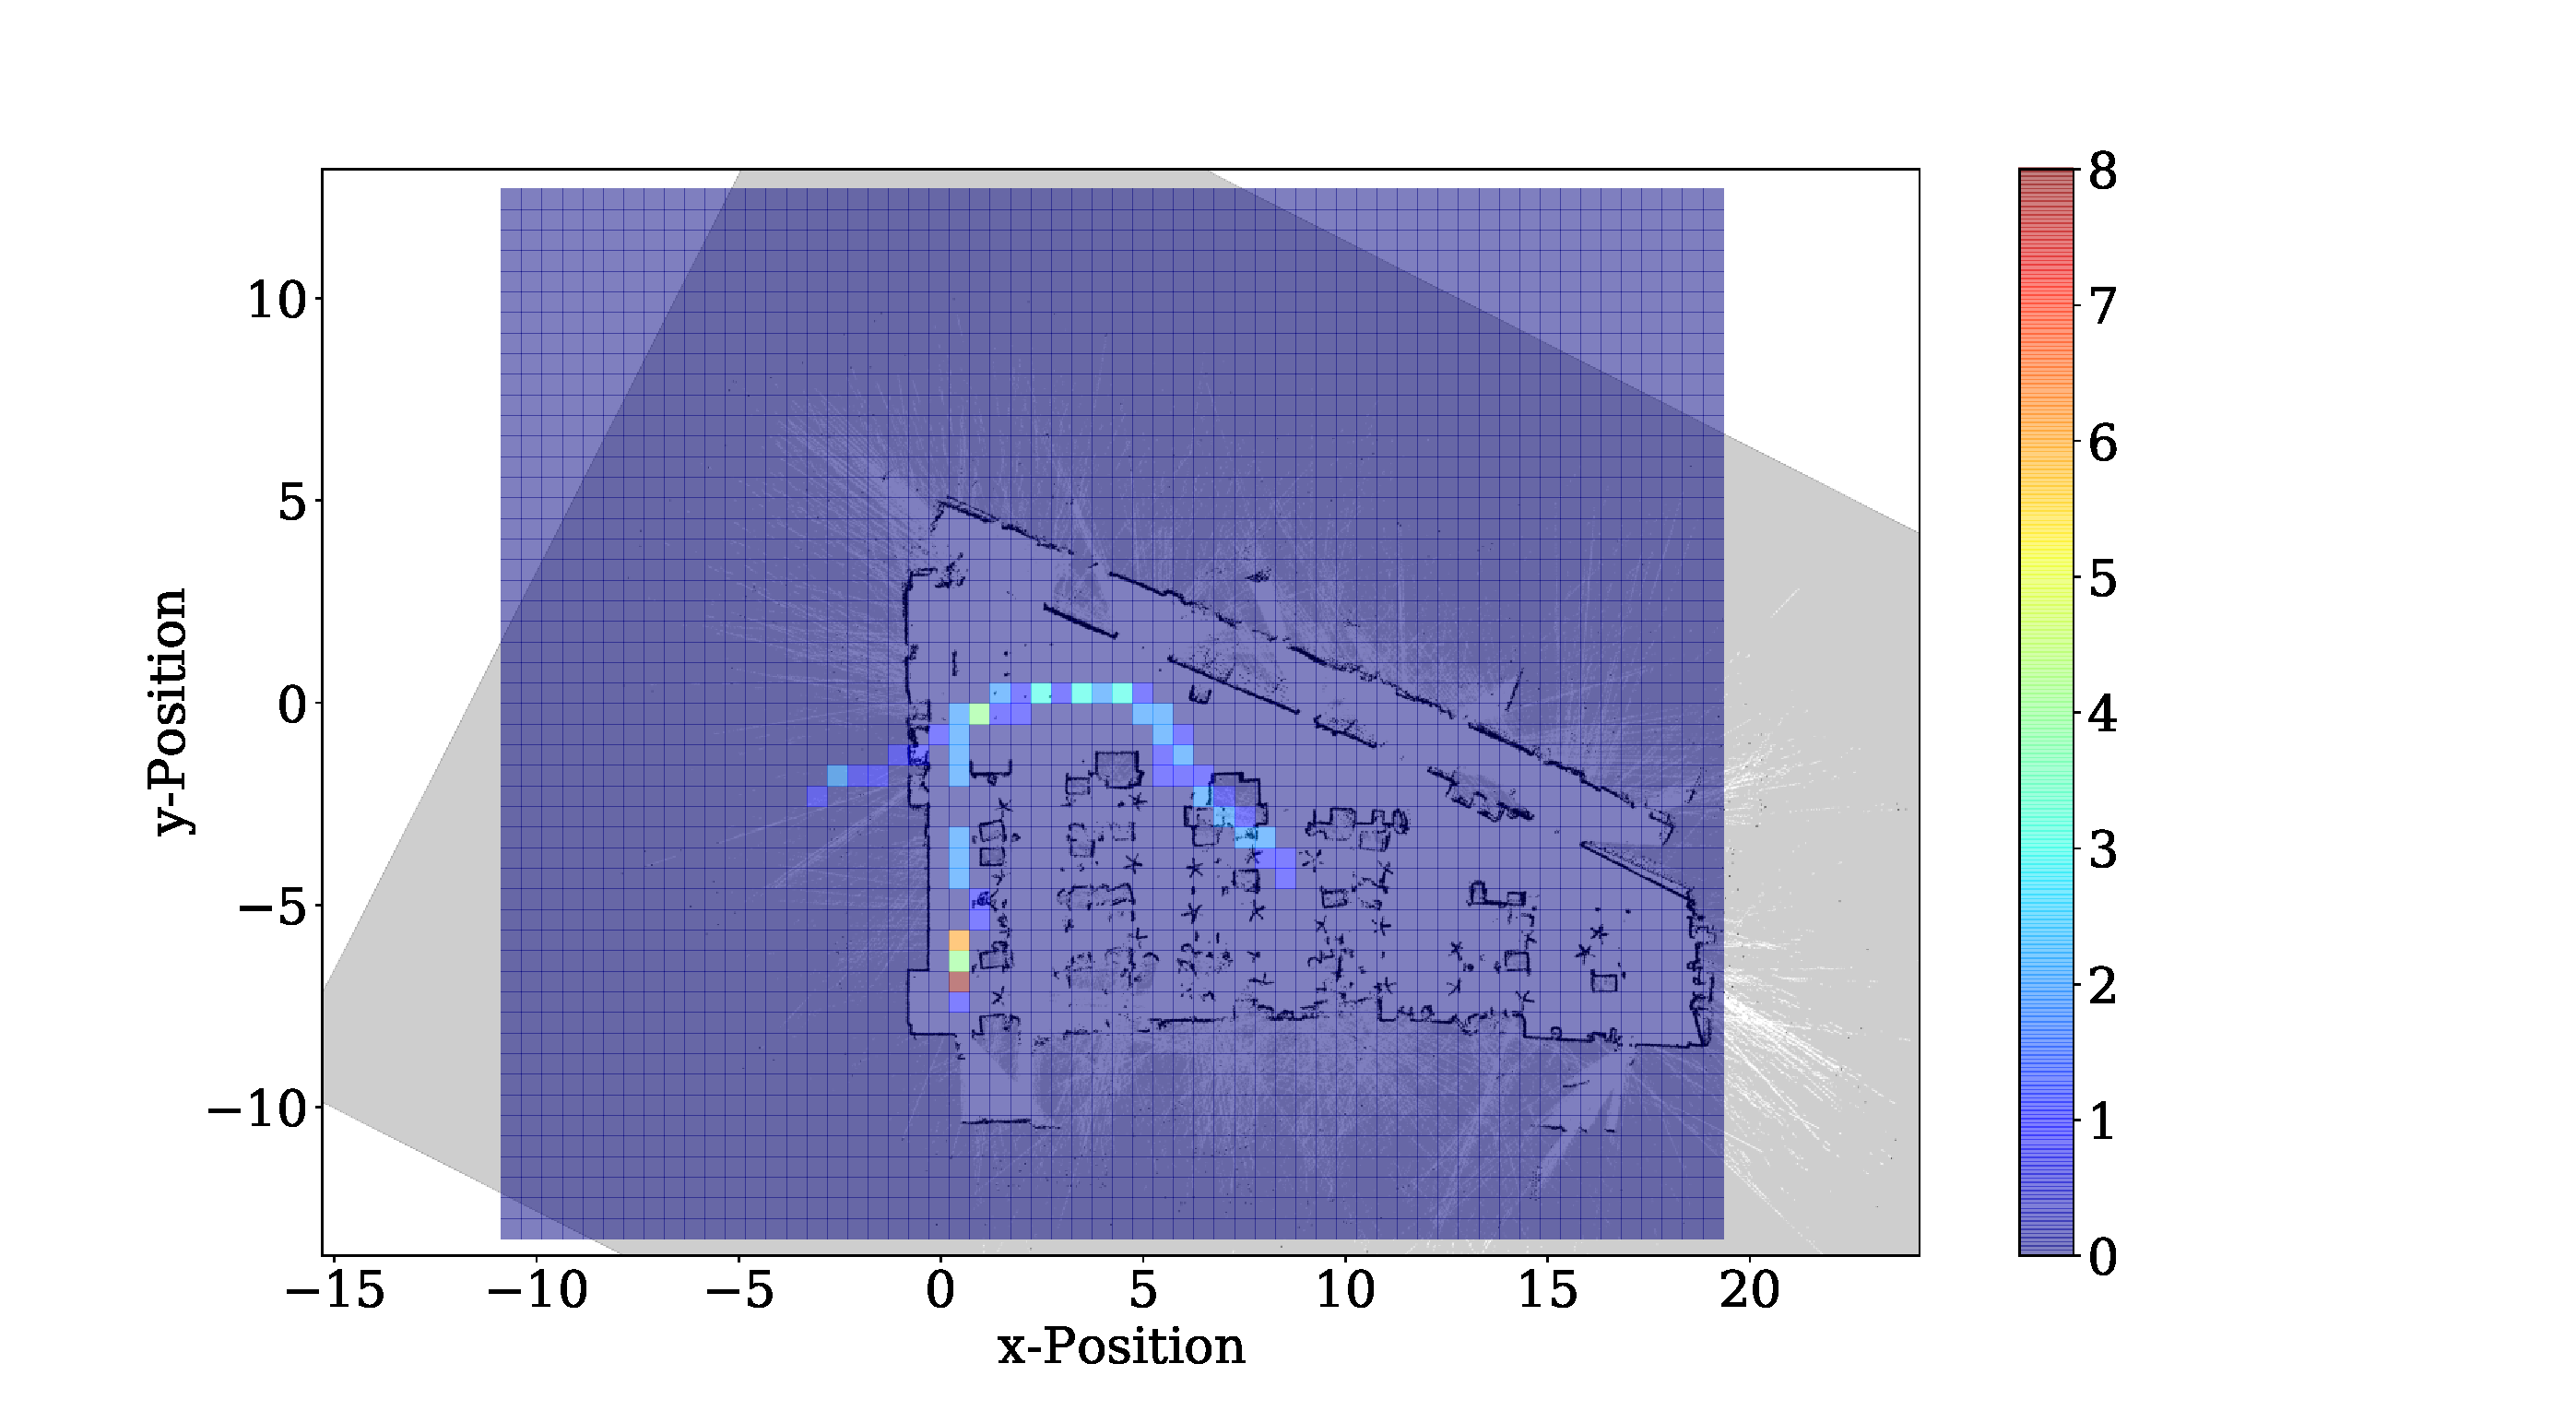
\includegraphics[width=\linewidth]{Abbildungen/methodik/Occupancy_grid_anschaulich}
		\caption[Belegungskarte grafische Darstellung]{Belegungskarte eines Bürogebäudes, über welches ein Gitter (blau) gelegt ist}
		\label{fig.Bürogebäude_Gitter}
	\end{center}
\end{figure}

Zu sehen sind hier die schematischen Umrisse eines Bürogebäudes. In blau dargestellt und über die Büroumrisse gelegt ist das oben beschriebene Gitter. Die Farbinformation spiegelt die Anzahl an Messdaten innerhalb der einzelnen Zellen wider. Eine Zelle ist dabei durch ihre x- und y-Position innerhalb des Umgebungskoordinatensystems $\textrm{(KS)}_\ind{\mathcal{U}}$ definiert. 
Ist die Umgebung $\mathcal{U}$ in einzelne Zellen unterteilt, lässt sich das oben beschriebene Gitter in Matrixschreibweise ausdrücken als
\begin{equation}
	\boldsymbol{G_\ind{Gitter}} = \begin{pmatrix}
		\boldsymbol{A}_{1,1} & \boldsymbol{A}_{1,2} &\hdots & \boldsymbol{A}_{1,n} \\
		\boldsymbol{A}_{2,1} & \boldsymbol{A}_{2,2} & \hdots & \boldsymbol{A}_{2,n} \\
		\vdots & \vdots & \ddots & \vdots \\
		\boldsymbol{A}_{n,1} & \boldsymbol{A}_{n,2} & \hdots & \boldsymbol{A}_{n,n}
	\end{pmatrix} .
\label{eq:Umgebungsmatrix}
\end{equation}

Hierbei bezeichnet $\boldsymbol{A}_{2,2}$ die Zelle der zweiten Reihe und der zweiten Spalte des Gitters, in welches die Umgebung eingeteilt wird. Es ist zu erwähnen, dass es sich um ein rechteckiges Gitter handelt, welches über die Umgebung $\mathcal{U}$ gelegt wird. Der Bereich einer Zelle $\boldsymbol{A}_{i,j}$ ist definiert durch ihre Grenzen $x_\ind{left}$ und $x_\ind{right}$ in x-Richtung, sowie die Grenzen $y_\ind{bottom}$ und $y_\ind{top}$ in y-Richtung des Umgebungskoordinatensystems $\textrm{(KS)}_\ind{\mathcal{U}}$. Eine Detektion $\boldsymbol{x}_i$ wird der Zelle $\boldsymbol{A}_{i,j}$ zugeordnet, sofern gilt 
\begin{equation}\label{eq:Grenzen einer Zelle}
	x_\ind{det} \in [x_\ind{left}, x_\ind{right}] \land y_\ind{det} \in [y_\ind{bottom}, y_\ind{top}] .
\end{equation}
Ein Eintrag in einer Zelle $\boldsymbol{A}_{i,j}$ besteht aus einem Tupel mit den Einträgen $(a, t_\ind{det})$. Der Parameter $a$ nimmt im Fall einer Personendetektion den Wert $1$ an, $t_\ind{det}$ beinhaltet die zeitliche Information der Personendetektion. Werden nach und nach mehr Detektionen innerhalb einer bestimmten Zelle getätigt, enthält die Zelle $\boldsymbol{A}_{i,j}$ eine Menge $\mathcal{L}$ bestehend aus $l$ Tupeln. Zeichnet man alle Detektionen für einen bestimmten Zeitraum, zum Beispiel für eine Woche auf, lassen sich die Messungen in Zeitintervalle $\Delta t_n$ unterteilen. Beträgt die Gesamtdauer des zum Aufzeichnen von Detektionen betrachteten Zeitraumes $T$, so ergibt sich die Gesamtzahl an Intervallen bei einer Intervalldauer von $\Delta t$ zu
\begin{equation}
	n_\ind{t} = \frac{T}{\Delta t} .
	\label{eq:Number timestamps}
\end{equation}
Die Dauer des Zeitraumes $T = t_b - t_a$ wird durch seinen Startzeitpunkt $t_a$ sowie seinen Endzeitpunkt $t_b$ definiert. Das $n$-te Zeitintervall $\Delta t_n$ befindet sich innerhalb der Grenzen $[t_a + n\Delta t,\, t_a + (n+1) \Delta t]$. Um die Übersichtlichkeit der Methodik weiterhin gewährleisten zu können, wird im Folgenden die Zelle $\boldsymbol{A}_{i,j}$ nur noch mit $\boldsymbol{A}$ bezeichnet. Um die Aktivität, beziehungsweise das Personenaufkommen in einer Zelle des Gitters bestimmen zu können, wird die Anzahl der Detektionen pro Zeitintervall aufsummiert. Die Summe an Detektionen in der Zelle $\boldsymbol{A}$ im $n$-ten Zeitintervall lässt sich schreiben als
\begin{equation}
	a_{n} = \sum_{k=1}^{K} l_k \in [t_a + n\Delta t, t_a + (n+1) \Delta t] ,
	\label{eq:Detektionen pro Intervall}
\end{equation}
wobei mit $K$ die Gesamtanzahl der Detektionen innerhalb des Gesamtzeitraumes $T$ bezeichnet wird.
Nach der Unterteilung des gesamten Zeitraumes in Intervalle und das Aufsummieren der Detektionen innerhalb dieser Intervalle enthält jede Zelle die Information des zeitlichen Verlaufes des Personenaufkommens innerhalb ihrer geografischen Grenzen. Die Zelle $\boldsymbol{A}$ und die in ihr enthaltene Information lässt sich schreiben als
\begin{equation}
	\boldsymbol{A} = (\boldsymbol{a}, \boldsymbol{t})^T .
	\label{eq:Vereinfachte Zellengleichung}
\end{equation}

Hierbei bezeichnet $\boldsymbol{a} = (a_1, a_2, \dots ,a_n)^T$ alle aufsummierten Personendetektionen innerhalb der Zeitintervalle mit den korrespondierenden Zeitstempeln $\boldsymbol{t} = (t_1, t_2, \dots ,t_n)^T$. Als Zeitstempel jeden Intervalls wird dessen Startzeitpunkt gewählt. Anschaulich beschrieben erhält man für jeden Zeitstempel die Information, wie viele Personen sich innerhalb des betreffenden Zeitintervalls in den Zellen des Gitters befunden haben. Für einen Betrachtungszeitraum mit $n$ Zeitstempeln ergibt sich eine dreidimensionale Matrix, auf dessen dritter Achse $n$ Matrizen $\boldsymbol{G}_\ind{Gitter}$ (vgl. Gleichung \ref{eq:Umgebungsmatrix}) hintereinander gestapelt werden. Im Falle des binären Zustandsmodells werden die Einträge jeder Zelle eines Zeitstempels durch die Werte $\{0,1\}$ abgebildet. Es wird lediglich das Vorhandensein einer Person innerhalb eines Zeitintervalls in einer Zelle registriert, nicht jedoch die Anzahl der Personen innerhalb des Zeitintervalls.
Ein qualitativer Vergleich der beiden Methoden kann durch \bild{occupancy_grid_vergleich} gezogen werden.

\begin{figure}[!h]
	\begin{center}
		\centering
		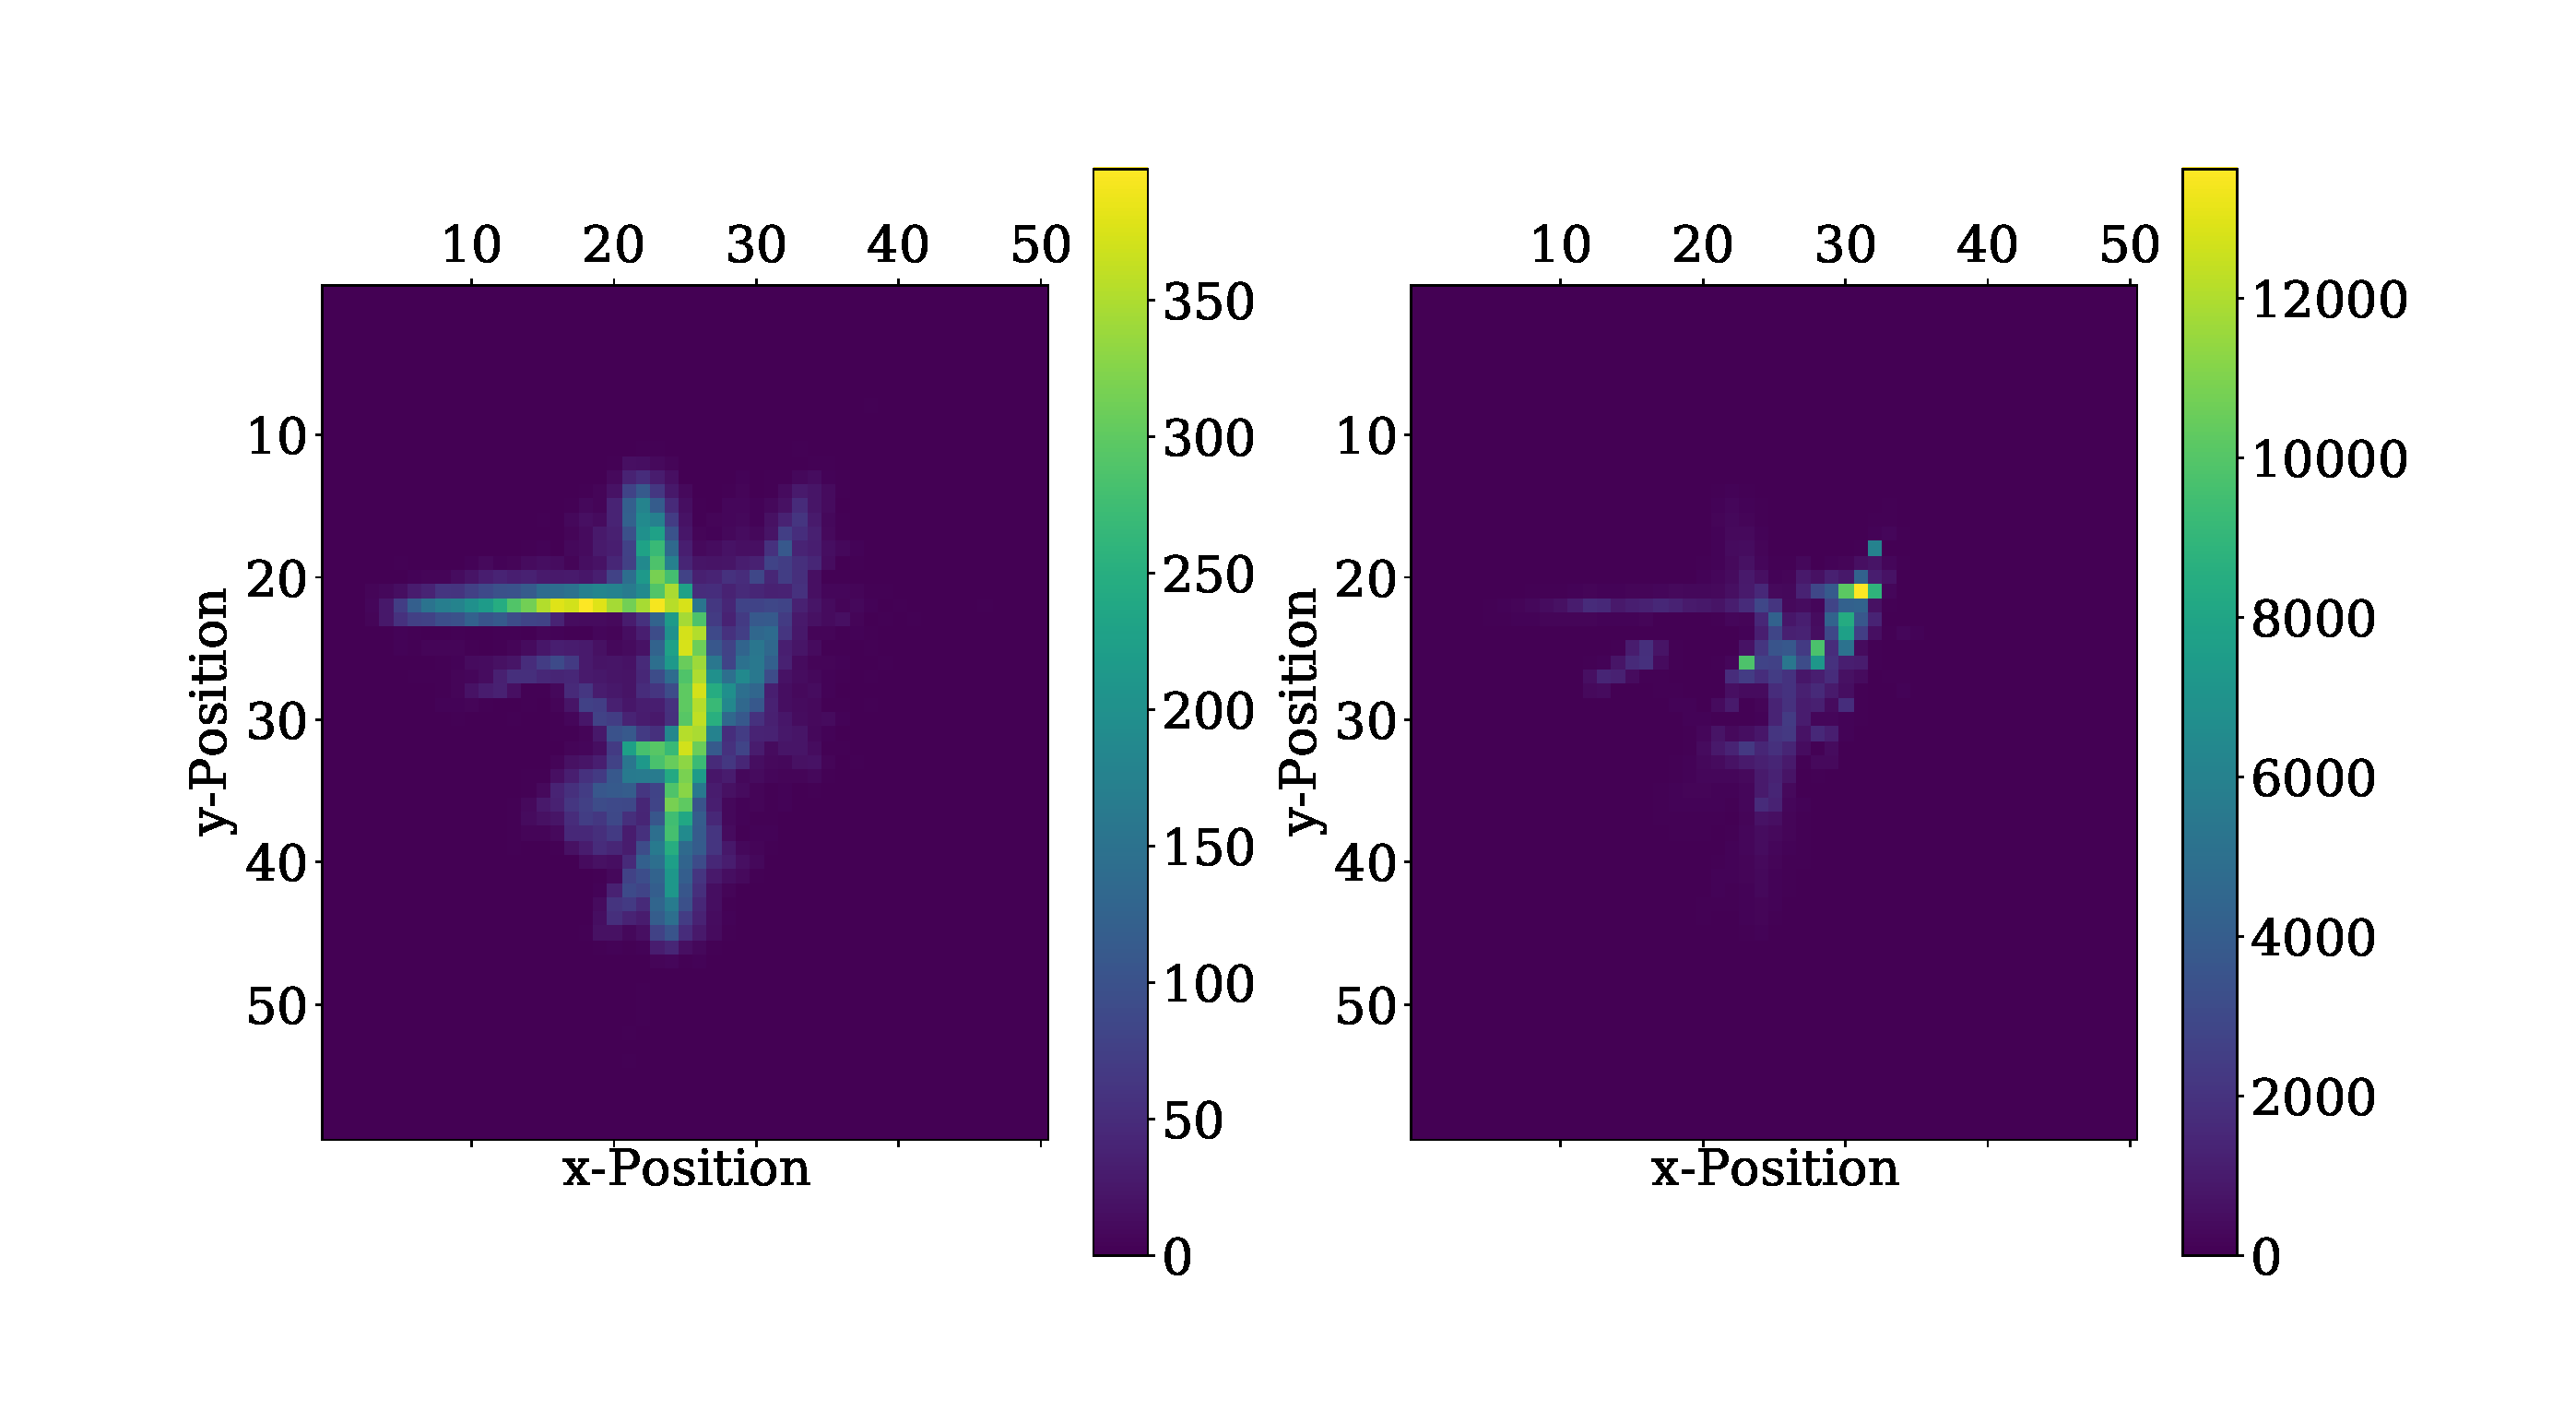
\includegraphics[width=1.0\linewidth]{Abbildungen/methodik/occupancy_grid_vergleich}
		\caption[Vergleich Personendetektion binärer und quantitativer Fall]{Aufsummierte Personendetektionen innerhalb eines Zeitraumes von einer Woche mit Beschränkung auf \{0, 1\} (links) und ohne Beschränkung (rechts)}
		\label{fig.occupancy_grid_vergleich}
	\end{center}
\end{figure}

Beiden Abbildungen liegen aufsummierte Personendetektionen innerhalb eines Zeitraumes von einer Woche mit der Aufteilung in Zeitintervalle von $\Delta t = \SI{600}{\second}$ zugrunde. Im linken Bild sieht man die Darstellung von Detektionen, welche pro Zeitintervall auf \{0,1\} beschränkt sind. Farblich hervorgehoben sind hier also Zellen, welche über viele Zeitintervalle hinweg häufig besucht wurden. Im rechten Bild dargestellt sind die nicht beschränkten, aufsummierten Personendetektionen. Farblich hervorgehoben sind hier die Zellen, welche innerhalb des gesamten Betrachtungszeitraumes am häufigsten besucht wurden, dies sich aber auf eine relativ kurze Zeitspanne innerhalb des Betrachtungszeitraumes beschränken kann. Im weiteren Verlauf dieses Kapitels wird lediglich der binäre Fall behandelt, also die auf \{0,1\} beschränkte Detektion von Personen innerhalb eines Zeitintervalls. Die so ermittelten Daten bilden einen Trend über den Betrachtungszeitraum ab. 
Die Unterteilung in Zeitintervalle ist der Tatsache geschuldet, dass in der Praxis das Wissen über die Zellzustände lückenhaft ist. Es kann lediglich durch, von einem mobilen Roboter durchgeführte, stichprobenartige Messungen approximiert werden. Mit einer größer werdenden Intervalldauer lassen sich die Messungen flexibler durchführen. Eine größere Intervalldauer geht jedoch mit einer stetig steigenden Verallgemeinerung des Zellzustandes und dem Verlust von Informationen einher. \\ 
Die registrierten Daten werden in einem weiteren Schritt in einer Datenbank gespeichert. Dies ermöglicht den externen Zugriff eines in Abschnitt \ref{sec.Verarbeitung client binär} behandelten Clients auf die Messdaten. Ein einzelner Eintrag in der Datenbank besitzt dabei immer den gleichen Aufbau. Neben dem Zellennamen werden der Zeitstempel sowie die Information, ob die Zelle im betrachteten Zeitintervall belegt oder frei war, gespeichert. 

\subsection{Verarbeitung der Messdaten Client-seitig}
\label{sec.Verarbeitung client binär}

Auf der Clientseite wird das Gitter $\boldsymbol{G}_\ind{Gitter}$ mit seinen Zelleinträgen $\boldsymbol{A}_{i,j}$ rekonstruiert. Hierzu greift der Client auf die in Abschnitt \ref{sec.Messdatenermittlung eines Belegtheitsgitters binär} beschriebene Datenbank zu und erstellt seinerseits ein Gitter, in welchem für jede Zelle eine Matrix, bestehend aus einem Vektor an Zeitstempeln und dem dazu korrespondierenden Vektor der Personendetektionen, nach Gleichung \ref{eq:Vereinfachte Zellengleichung} angelegt wird.
Der Zustand jeder einzelnen Zelle des Gitters ist als Funktion der Zeit innerhalb des Clients gespeichert und lässt sich nach \cite{Krajnik.2014} als $s(t)$ schreiben. Da auch in dieser Arbeit von dem Ansatz ausgegangen wird, dass das menschliche Verhalten, also auch das örtliche Auftreten von Personen, gewissen zeitlichen Periodizitäten unterliegt, werden die Daten der einzelnen Zellen im Folgenden an einen Server geschickt, auf welchem Untersuchungen ihrer Frequenzspektren erfolgen.

\begin{figure}[!h]
	\begin{center}
		\centering
		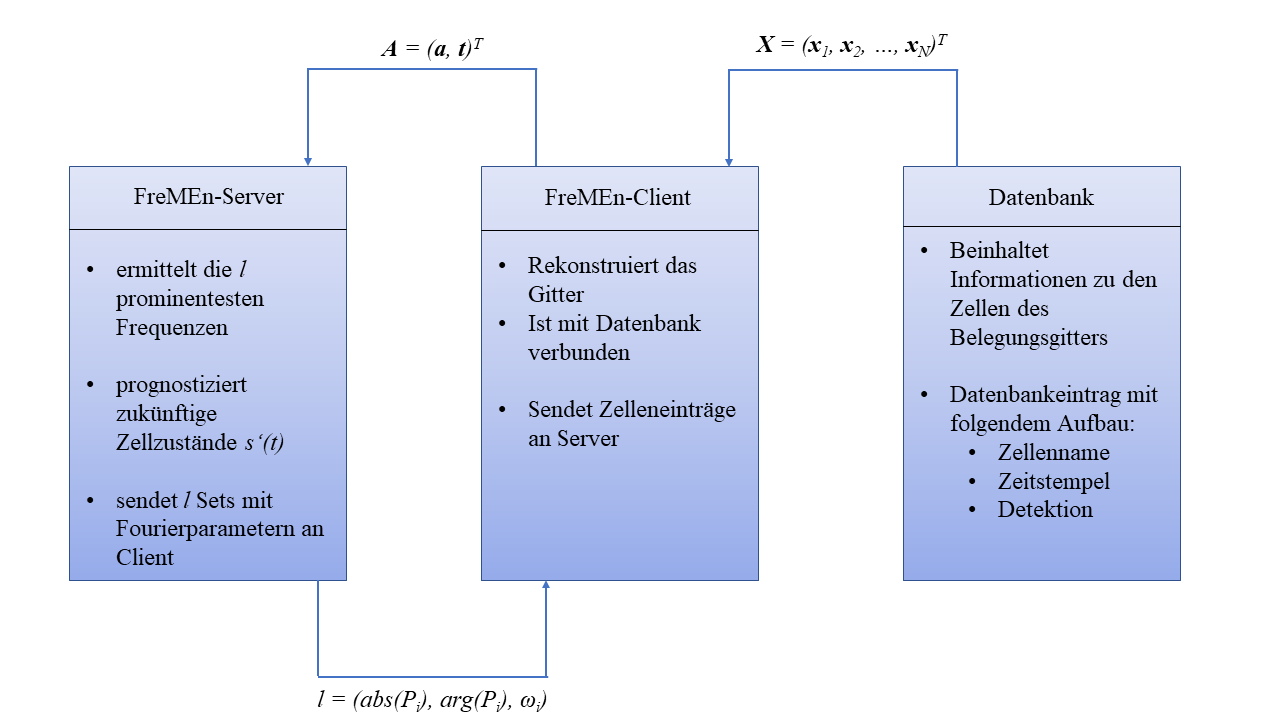
\includegraphics[width=1.0\linewidth]{Abbildungen/methodik/Ablauf_binaer}
		\caption[Informationsfluss binäres Modell]{Informationsfluss binäres Modell}
		\label{fig.Informationsfluss_binäres_Modell}
	\end{center}
\end{figure}


\subsection{Verarbeitung der Messdaten Server-seitig}
\label{sec.Verarbeitung server binär}

Der Server erstellt für jede Zelle des Belegtheitsgitters ein Modell. Als Eingang dienen dem Server die von dem Client gesendeten Datenarrays der einzelnen Zellen mit den Zeitstempeln und den dazu gehörigen Belegtheitsinformationen. Da die Zellen als linear unabhängig betrachtet werden, wird für jede Zelle ein eigenes Modell erstellt. Als Eingangsgröße dient, wie schon in \cite{Krajnik.2014}, die Belegtheit der Zelle als Funktion von der Zeit $s(t)$. Es sei darauf hingewiesen, dass $s(t)$ keine kontinuierliche, sondern eine diskrete, binäre Funktion mit Einträgen zu den Zeitpunkten der Zeitstempel ist. Die Funktion $s(t)$ soll durch eine Wahrscheinlichkeitsfunktion $p(t)$ approximiert werden. Das Vorgehen entspricht der Frequency-Map-Enhancement (FreMEn) Methode aus \cite{Krajnik.2015b}. Das Frequenzspektrum der Funktion $s(t)$ soll ermittelt werden. Hierzu wird eine inkrementelle Fouriertransformation des Zustandsvektors $s(t)$ durchgeführt mit 

\begin{equation}\label{eq:Inkrementelle Fouriertransformation} 
	\begin{split} 
		\mu &\leftarrow \frac{1}{n+1} (n \mu + s(t)) ,\\ 
		\alpha_k &\leftarrow \frac{1}{n+1} (n \alpha_k + s(t) e^{-jt \omega_k}) ,\qquad \forall \omega_k \in \Omega ,\\ 
		\beta_k &\leftarrow \frac{1}{n+1} (n \beta_k + \mu e^{-j \omega_k}) ,\qquad \quad \, \, \forall \omega_k \in \Omega ,\\ 
		n &\leftarrow n + 1 .
	\end{split} 
\end{equation} 

Gleichung \ref{eq:Inkrementelle Fouriertransformation} gleicht dem Vorgehen aus \cite{Krajnik.2015}. Mit jeder neuen Detektion werden die Werte aktualisiert. Zur Erinnerung sei darauf hingewiesen, dass die Grundidee dieser Methode darin besteht, die zeitliche Zustandsfunktion $s(t)$ jeder Zelle des Gitters durch eine Wahrscheinlichkeitsfunktion $p(t)$ zu approximieren, welcher $l$ periodische Prozesse zugrunde liegen. Die Zustandsfunktion jeder Zelle wird dabei durch die Zellzustände zu den Zeitstempeln $t_1, t_2, \dots , t_n$,\, ihren Durchschnittswert $\mu$, und zwei Mengen $\mathcal{A}, \mathcal{B}$ komplexer Zahlen $\alpha_k$ und $\beta_k$ des korrespondierenden periodischen Prozesses mit der Frequenz $\omega_k$ aus der Menge $\Omega$ beschrieben. Initialisiert wird jede Zelle mit dem Durchschnittswert $\mu = 0.5$, alle Werte $\alpha_k, \beta_k$ werden zu 0 gesetzt. Der Betrag $\gamma_k = |\alpha_k - \beta_k |$ entspricht dem durchschnittlichen Einfluss des periodischen Prozesses mit der Frequenz $\omega_k$ auf den Zellzustand $s(t)$. \\
Im Gegensatz zu \cite{Krajnik.2015} wird im Vorhinein eine feste Periodendauer $T$ von beispielsweise einer Woche vorgegeben. Da die Observationen innerhalb diskreter, über den Zeitraum $T$ gleichmäßig verteilter Intervalle $\Delta t$ erfolgen, vereinfacht sich Gleichung \ref{eq:Inkrementelle Fouriertransformation} formal zur traditionellen Diskreten Fouriertransformation (DFT). Die Informationen über den Zellzustand $s(t)$ werden, wie in Abschnitt \ref{sec.Messdatenermittlung eines Belegtheitsgitters binär} beschrieben, innerhalb einer Datenbank gespeichert. Beträgt die Gesamtdauer der in der Datenbank gespeicherten Daten $n$ mal $T$, sind also $n$ Samples der a priori definierten Periodendauer $T$ gegeben, so erfolgt eine Mittelung der Werte innerhalb korrespondierender Zeitintervalle $\Delta t_i$ durch \\

\begin{equation}\label{eq:Mittelung Fourierkoeffizienten}
	\begin{split}
		\bar{\mu} &= \frac{1}{n} \sum_{i=1}^{n} \mu_i ,	\\
		\bar{\alpha}_k &= \frac{1}{n} \sum_{i=1}^{n} \alpha_{k,i} ,\\
		\bar{\beta}_k &= \frac{1}{n} \sum_{i=1}^{n} \beta_{k,i} .
	\end{split}
\end{equation} 

Die Wahrscheinlichkeitsfunktion $p(t)$ des Zellzustandes $s(t)$ wird wie in \cite{Krajnik.2015} mittels Extraktion der $l$ periodischen Prozesse mit den höchsten Amplituden $\bar{\gamma}_k = | \bar{\alpha}_k - \bar{\beta}_k | $ gebildet. Nach deren Überlagerung ergibt sich die Wahrscheinlichkeitsfunktion $p(t)$ zu

\begin{equation}\label{eq:Zellzustands-Wahrscheinlichkeitsfunktion}
	p(t) = \zeta (\bar{\mu} + \sum_{l=1}^{m} |\bar{\gamma}_l| \cos(\omega_k t + \mathrm{arg}(\bar{\gamma}_l))) .
\end{equation}

Hierbei versichert $\zeta (.) $, dass die Funktion $p(t) \in [0, 1]$ ist. Zur Erläuterung sei angemerkt, dass, obwohl die Werte von $s(t)$ im hier betrachteten binären Fall lediglich die Zustände $\{0, 1\}$ annehmen können, die durch Fouriertransformation und inverse Fouriertransformation ermittelte Funktion $p(t)$ Werte größer als $1$ annehmen kann. \\
Die Berechnung von $p(t)$ durch Gleichung \ref{eq:Zellzustands-Wahrscheinlichkeitsfunktion} erlaubt es, zukünftige Zustände $s(t)$ einer Zelle zu ermitteln. Ein beliebiger Zeitpunkt $t$ wird dazu auf dem entsprechenden Zeitintervall $\Delta t_n$ innerhalb des Gesamtzeitraumes $T$ abgebildet. Die Vorhersage $s'(t)$ des Zellzustandes erfolgt mittels eines Schwellwertes $c$ zu

\begin{equation}\label{eq:Schwellwert-Verfahren}
	{s'}_i (t) = \begin{cases}
		1 & \, , \qquad p(t) \geq c \\
		0 & \, , \qquad p(t) < c 
	\end{cases} .
\end{equation}

Zur Ermittlung der optimalen Anzahl $l_\ind{opt}$ an periodischen Prozessen zur Bestimmung der Wahrscheinlichkeitsfunktion $p(t)$ wird auf die Einteilung des Datensatzes in ein \glqq{Estimation-Set}\grqq{} sowie ein \glqq{Prediction-Set}\grqq{} eingegangen. Ist die Gesamtdauer der in der Datenbank vorhandenen Zelleinträge $T$, so werden zur Berechnung der Modellkoeffizienten nach Gleichung \ref{eq:Inkrementelle Fouriertransformation} Daten innerhalb des Zeitintervalls $\Delta T_\ind{Est}$ verwendet. Der Schätzfehler $\epsilon_\ind{r} (T)$, also die Genauigkeit, mit der das Modell die zu seiner Erstellung verwendeten Daten rekonstruieren kann, ergibt sich zu

\begin{equation}\label{eq:Schätzfehler}
	\epsilon_\ind{r}(\Delta T_\ind{Est}) = \frac{1}{n} \sum_{i=1}^{n} |s_i '(t) - s_i (t)| .
\end{equation}

Alle zur Berechnung des Fehlers $\epsilon_\ind{r}$ verwendeten Daten müssen innerhalb des Intervalls $\Delta T_\ind{Est}$ liegen. \\
Das Zeitintervall $\Delta T_\ind{Pred}$ beinhaltet Messungen, welche nicht zur Erstellung des Modells verwendet wurden. Der Fehler $\epsilon_\ind{p}$ beschreibt, wie genau das Modell zukünftige Zustände einer Zelle vorhersagen kann. Der Fehler $\epsilon_\ind{p}$ berechnet sich als

\begin{equation}
	\label{eq:Prädiktionsfehler}
		\epsilon_\ind{p}(\Delta T_\ind{Pred}) = \frac{1}{n} \sum_{i=1}^{n} |s_i '(t) - s_i (t)| ,
	\end{equation}
	
mit allen Messwerten innerhalb des Intervalls $\Delta T_\ind{Pred}$. Die optimale Modellordnung $l_\ind{opt}$ wird nach \cite{Krajnik.2015} so gewählt, dass der Prädiktionsfehler $\epsilon_\ind{p}$ minimiert wird. Die maximale Modellordnung wird zu $l_\ind{max} = 20$ gesetzt. \\

\section{Quantitative Zustandsmodelle}
\label{sec.Quantitative Zustandsmodelle}
Um Aussagen über die Anzahl an Ereignissen innerhalb eines Zeitintervalls treffen zu können, kann dies, wie schon in Abschnitt \ref{sec.Beschreibung quantitativer Zustandsmodelle} erwähnt, mittels quantitativer Zustandsmodelle erreicht werden. Es sollen Schätzungen $\lambda'(t)$ für die, intervallweise definierte, Funktion $\lambda(t)$ einer Aktivitätenrate berechnet werden. Hierzu folgt in einem ersten Schritt die Ermittlung von Messdaten eines Belegtheitsgitters (Abschnitt \ref{sec.Messdatenermittlung quantitativ}), bevor diese Daten Client-seitig verarbeitet werden (Abschnitt \ref{sec.Messdatenverarbeitung client quantitativ}). In einem weiteren Schritt werden die Daten an einen Server gesendet, welcher für jede Zelle des Belegtheitsgitters ein quantitatives Zustandsmodell erstellt (Abschnitt \ref{sec.Messdatenverarbeitung server quantitativ}).
\subsection{Messdatenermittlung eines Belegtheitsgitters}
\label{sec.Messdatenermittlung quantitativ}

Wie schon in Abschnitt \ref{sec.Binäre Zustandsmodelle} wird auch in diesem Abschnitt, welcher quantitative Zustandsmodelle behandelt, ein Gitter über eine Umgebung $\mathcal{U}$ gelegt, und für einen Betrachtungszeitraum $T$, unterteilt in $n$ Intervalle mit der Intervalldauer $\Delta t$, die Personendetektionen innerhalb der Zellen gezählt. Die Methodik gleicht der des binären Modells, jedoch erfolgt keine Beschränkung der Detektionen pro Intervall auf \{0,1\}. Die Einträge einer einzelnen Zelle des Gitters werden geschrieben als
\begin{equation}
	\boldsymbol{A} = (\boldsymbol{\lambda}, \boldsymbol{t})^T .
	\label{eq:Zelleinträge quantitativer Fall}
\end{equation}

Da im quantitativen Fall die Anzahl an Personen pro Zeitintervall $\Delta t$, also die Personenrate gezählt wird, enthält Gleichung \ref{eq:Zelleinträge quantitativer Fall} die Personenraten $\boldsymbol{\lambda} = (\lambda_1, \lambda_2, \dots , \lambda_n)^T$ \, der einzelnen Zeitintervalle sowie die Zeitstempel $\boldsymbol{t} = (t_1, t_2, \dots , t_n)^T$ \, der zugehörigen Intervalle. Eine Erhöhung der Intervalldauer $\Delta t$ geht dabei mit steigenden Einträgen der Personenraten $\boldsymbol{\lambda}$ und einem Informationsverlust einher. \\
Die registrierten Daten werden, wie schon in Abschnitt \ref{sec.Messdatenermittlung eines Belegtheitsgitters binär}, in einer Datenbank gespeichert. Ein Datenbankeintrag enthält neben dem Zellennamen den Zeitstempel des Zeitintervalls sowie die zugehörige Personenrate $\lambda$.

\subsection{Verarbeitung der Messdaten Client-seitig}
\label{sec.Messdatenverarbeitung client quantitativ}

Die Verarbeitung der Messdaten auf der Clientseite gleicht dem Vorgehen in Abschnitt \ref{sec.Verarbeitung client binär}. Das Gitter $\boldsymbol{G}_\ind{Gitter}$ mit seinen Zelleinträgen $\boldsymbol{A}_{i,j}$ wird rekonstruiert. Jede rekonstruierte Zelle enthält einen Vektor $\boldsymbol{t}$ an Zeitstempeln und den Vektor $\boldsymbol{\lambda}$ der Personenraten der einzelnen Zeitintervalle. Die beiden Vektoren jeder Zelle werden im nächsten Schritt an den Server geschickt, auf welchem Untersuchungen der Frequenzspektren der Zelle erfolgen.

\begin{figure}[!h]
	\begin{center}
		\centering
		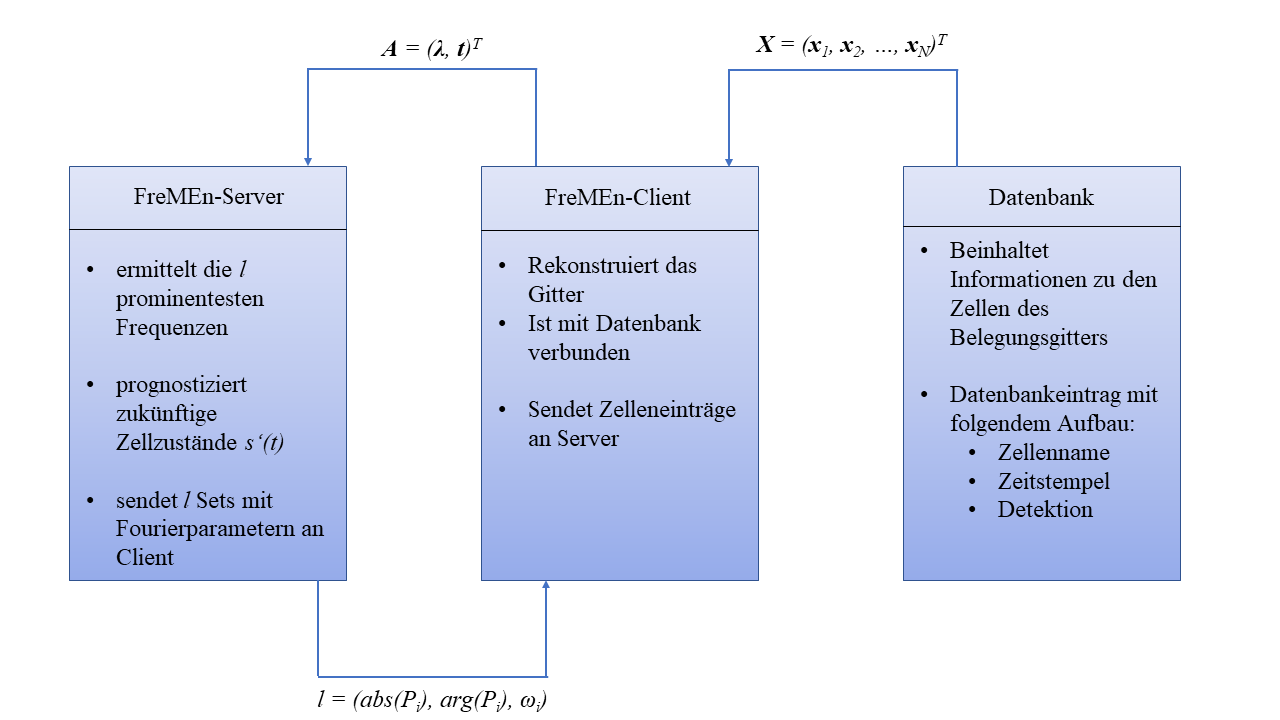
\includegraphics[width=1.0\linewidth]{Abbildungen/methodik/Ablauf_quantitativ}
		\caption[Informationsfluss quantitatives Modell]{Informationsfluss quantitatives Modell}
		\label{fig.Informationsfluss_quantitatives_Modell}
	\end{center}
\end{figure}

\subsection{Verarbeitung der Messdaten Server-seitig}
\label{sec.Messdatenverarbeitung server quantitativ}

Wie schon in Abschnitt \ref{sec.Verarbeitung client binär} erstellt der Server auch für den quantitativen Fall für jede Zelle des Belegtheitsgitters ein Modell. Wieder wird aufgrund der linearen Unabhängigkeit der Zellen für jede einzelne Zelle ein eigenes Modell erstellt. Als Eingangsgröße dient, wie in \cite{Jovan.2016}, die Personenrate $\lambda (t)$ als Funktion der Personenraten der einzelnen Zeitintervalle $\Delta t$. Die Funktion $\lambda (t)$ soll durch eine Funktion $\lambda ' (t)$ approximiert werden. Nach \cite{Krajnik.2015b} erfolgt eine inkrementelle Fouriertransformation der Personenraten-Funktion $\lambda (t)$ durch Gleichung \ref{eq:Inkrementelle Fouriertransformation}. Liegen in der Datenbank insgesamt $n$ Samples der a priori definierten Periodendauer $T$ vor, so erfolgt eine Mittelung der Werte korrespondierender Zeitintervalle $\Delta t_i$ nach Gleichung (\ref{eq:Mittelung Fourierkoeffizienten}). Die Approximation $\lambda ' (t)$ der Personenraten-Funktion $\lambda (t)$ ergibt sich zu
\begin{equation}\label{eq:Personenraten-Funktion}
	\lambda ' (t) = \zeta (\bar{\mu} + \sum_{l=1}^{m} |\bar{\gamma}_l| \cos(\omega_k t + \mathrm{arg}(\bar{\gamma}_l))) .
\end{equation} 

Hierbei versichert $\zeta (.) $, dass die Funktion $\lambda ' (t)$  den  Wert der am nächsten liegenden, natürlichen Zahl, annimmt. 
Zur Ermittlung der optimalen Anzahl $l_\ind{opt}$ an periodischen Prozessen zur Bestimmung der Personenraten-Funktion $\lambda (t)$ wird der Datensatz in ein \glqq{Estimation-Set}\grqq{} sowie ein \glqq{Prediction-Set}\grqq{} eingeteilt. Der Schätzfehler $\epsilon_\ind{r} (T)$, also die Genauigkeit, mit der das Modell die zu seiner Erstellung verwendeten Daten rekonstruieren kann, berechnet sich durch
\begin{equation}\label{eq:Schätzfehler quantitativ}
	\epsilon_\ind{r}(\Delta T_\ind{Est}) = \frac{1}{n} \sum_{i=1}^{n} |\lambda_i '(t) - \lambda_i (t)| .
\end{equation}
Alle zur Berechnung des Fehlers $\epsilon_\ind{r}$ verwendeten Daten müssen innerhalb des Intervalls $\Delta T_\ind{Est}$ liegen. \\
Das Zeitintervall $\Delta T_\ind{Pred}$ beinhaltet Messungen, welche nicht zur Erstellung des Modells verwendet wurden. Somit beschreibt der Fehler $\epsilon_\ind{p}$ wie schon in Abschnitt \ref{sec.Messdatenverarbeitung server quantitativ}, wie genau das Modell zukünftige Personenraten einer Zelle vorhersagen kann. Der Fehler $\epsilon_\ind{p}$ beträgt
\begin{equation}\label{eq:Prädiktionsfehler quantitativ}
	\epsilon_\ind{p}(\Delta T_\ind{Pred}) = \frac{1}{n} \sum_{i=1}^{n} |\lambda_i '(t) - \lambda_i (t)| ,
\end{equation}
mit allen Messwerten innerhalb des Intervalls $\Delta T_\ind{Pred}$. Die optimale Modellordnung $l_\ind{opt}$ wird so gewählt, dass der Prädiktionsfehler $\epsilon_\ind{p}$ minimiert wird. Die maximale Modellordnung wird zu $l_\ind{max} = 20$ gesetzt.